% !TeX root = ../main.tex
% **************************************************************************
\xchapter{基于图生成建模的视觉问答分布外泛化方法}{X-GGM: Graph Generative Modeling for Out-of-Distribution in Visual Question Answering}

近年来视觉问答任务取得了巨大的进展,但要使视觉问答模型能够自适应地泛化到分布外的样本仍然具有挑战性。直觉上,图像中已有的视觉概念(即目标和目标的属性)的重新组合可以产生在训练集中未见过的和罕见的组合,这些新的组合为视觉问答模型的分布外泛化提供了可能。
本章将视觉问答模型的分布外泛化问题表述为组合泛化问题,并提出了一种基于图生成建模的训练策略。
该策略利用图生成建模为预定义的以图像中目标-属性对作为节点的图迭代地生成关系矩阵和节点表征,来促进视觉问答模型泛化到分布外的样本。
此外,本章提出了一种梯度分布一致性损失来约束具有对抗性扰动的数据分布和生成的分布,有效地缓解了图生成建模过程中的训练不稳定问题。
在两个标准视觉问答分布外泛化评测数据集上的大量实验证明了本章提出的训练策略能显著提升视觉问答模型的分布外泛化能力,一定程度上解决了当前视觉问答模型因语言偏见导致的泛化能力不足的问题。



% **************************************************************************
\xsection{引言}{Introduction}

视觉问答~\cite{antol2015vqa}是指基于对图像的理解回答以自然语言形式给定的与图像内容有关的问题。
虽然视觉问答任务已取得了诸多先进进展,但当前大多数方法通常处理具有相似数据分布的训练集和测试集,这导致模型性能很大程度上会受到数据中的虚假相关~\cite{zhang2016yin,agrawal2016analyzing,goyal2017making,agrawal2018don}的影响。
然而,实用的视觉问答模型应该对答案分布的变化~\cite{kervadec2021roses} 具有鲁棒性并能在分布外(Out-of-Distribution, OOD)测试~\cite{teney2020value}中表现良好,即视觉问答模型对数据集特定语言偏见~\cite{agrawal2016analyzing,zhang2016yin,goyal2017making,agrawal2018don} 具有很好的泛化能力。
因此,为促进视觉问答的实用性,本章关注视觉问答任务的分布外泛化问题,旨在提高基线视觉问答模型的分布外泛化能力。

当前主流的提高视觉问答模型分布外泛化性能的方法以消除语言偏见为目标,可以简单地分为基于已知偏见的方法~\cite{clark2019don,chen2020counterfactual,liang2020learning} 和基于未知偏见的方法~\cite{teney2020unshuffling,gokhale2020mutant,clark2020learning}。
基于已知偏见的方法需要预先获取存在于特定数据集中语言偏见的统计信息,而基于未知偏见的方法旨在消除语言偏见或答案分布的变化而不需要事先知道偏见。
因此,基于未知偏见的方法更实用,但也更具挑战。
因为视觉问答模型要通过学习域内数据中的规则来生成未见过的或罕见的答案,即直接赋予视觉问答模型对分布外的样本进行泛化的潜力,才能自适应地泛化到任务样本。


人类因具有良好的组合泛化能力可以轻松实现分布外泛化~\cite{lake2017building}。
受此启发,本章将视觉问答的分布外泛化问题表述为组合泛化问题,并利用域内数据来生成现有视觉概念(目标和目标的属性)的新组合来促使视觉问答模型产生分布外的答案。
如图~\ref{fig:c3_motivation}所示,给定任意两组目标-属性对,如图~\ref{fig:c3_1} 中的绿色的西兰花(green broccoli)和棕色的食物(brown food),利用图生成建模即可得到新的组合,如图~\ref{fig:c3_2} 中的棕色的西兰花(brown broccoli)。
大量的新组合中就可能包含训练集中没有的或罕见的样本,这些样本则可以促进视觉问答模型泛化到分布外样本。
最新的工作~\cite{dai2018adversarial,zheng2020distribution}已经证明图生成模型~\cite{wang2018graphgan}有可能提高模型的泛化能力。
因此,本章使用图来表示视觉概念之间的关系,并在图生成建模过程中用已有视觉概念生成新的组合。



% ********************************************************************
\begin{figure}[!t]
\begin{subfigure}[b]{0.495\textwidth}
\centering
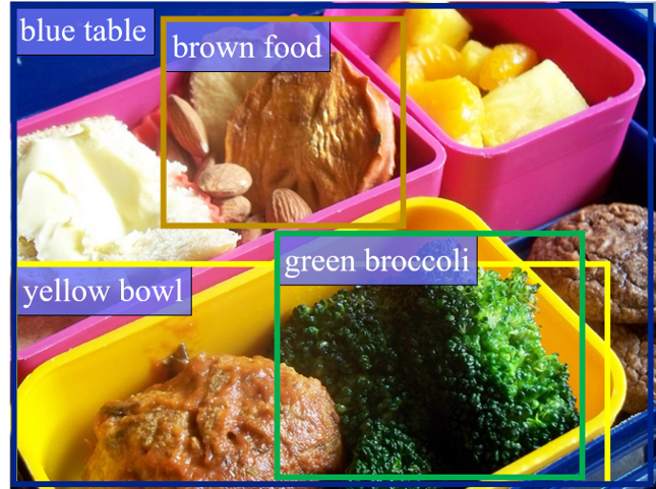
\includegraphics[height=5.3cm]{figure/c3_f1.png}
\subcaption{原始组合}
\label{fig:c3_1}
\end{subfigure}
\begin{subfigure}[b]{0.495\textwidth}
\centering
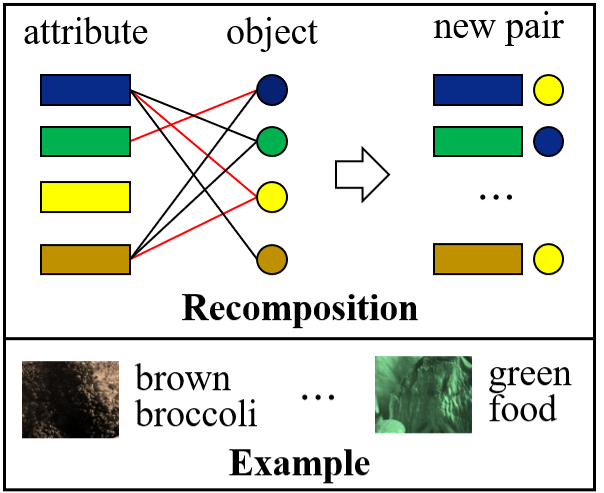
\includegraphics[height=5.3cm]{figure/c3_f2.png}
\subcaption{生成组合}
\label{fig:c3_2}
\end{subfigure}
\caption{图生成建模过程中蕴涵的组合泛化}
\label{fig:c3_motivation}
\end{figure}
% ********************************************************************


具体来说,本章提出了一种基于图生成建模的训练策略(X-Graph Generative Modeling,X-GGM)来提高现有视觉问答模型的分布外泛化性能。
如图~\ref{fig:c3_overview}所示,X-GGM具有两个核心模块:图关系的生成建模(Graph Relation Generative Modeling, R-GGM)和图表征的生成建模(Graph Representation Generative Modeling, N-GGM)。R-GGM旨在生成节点之间新的关系来间接地提高分布外泛化能力。它首先向跨模态表征$\xv$中引入对抗性扰动(即高斯噪声)来初始化关系矩阵。
然后,R-GGM利用图编码器聚合不同节点的信息并以迭代的方式更新关系矩阵。N-GGM的目标是生成新的节点表征来直接增强分布外泛化能力。
在N-GGM中,对抗扰动首先被添加到跨模态表征中来初始化节点表征。然后,图编码器被用于编码节点表征和生成新的节点表征。
X-GGM将对抗性扰动引入到跨模态表征中来刻画关系矩阵或节点表征的原始数据分布,这会导致图生成建模中的先验分布不准确的问题。不准确的分布会影响图对抗性学习的稳定性。
为了缓解训练的不稳定问题,本章提出了一个梯度分布一致性损失。该损失可以有效地约束输入对抗性扰动的数据分布和生成的分布(即生成的关系矩阵或节点表征的分布)之间的梯度一致性。因此,本章使用提出的梯度分布一致性损失代替图对抗学习中的重建损失来规避不准确先验分布的问题。

本章的主要贡献概括如下:
\begin{itemize}
\item 将视觉问答模型的分布外泛化问题表述为组合泛化问题,并提出了一种全新的基于图生成建模的训练策略。该策略在图生成建模过程中用已有视觉概念生成新的组合,显著地提高了现有视觉问答模型的分布外泛化能力。
\item 提出了一种新的梯度分布一致性损失。该损失在图生成建模过程中通过约束有对抗性扰动的数据分布和生成数据分布的梯度一致性,有效地缓解了图对抗性学习中的训练不稳定问题。
% \item 使用本章提出的X-GGM策略训练基线视觉问答模型(LXMERT)在VQA-CP v2和GQA-OOD数据上取得了最优的分布泛化外性能。广泛的消融实验证明了X-GGM组件的有效性。
\end{itemize}


% ********************************************************************
\begin{figure}[!t]
\centering
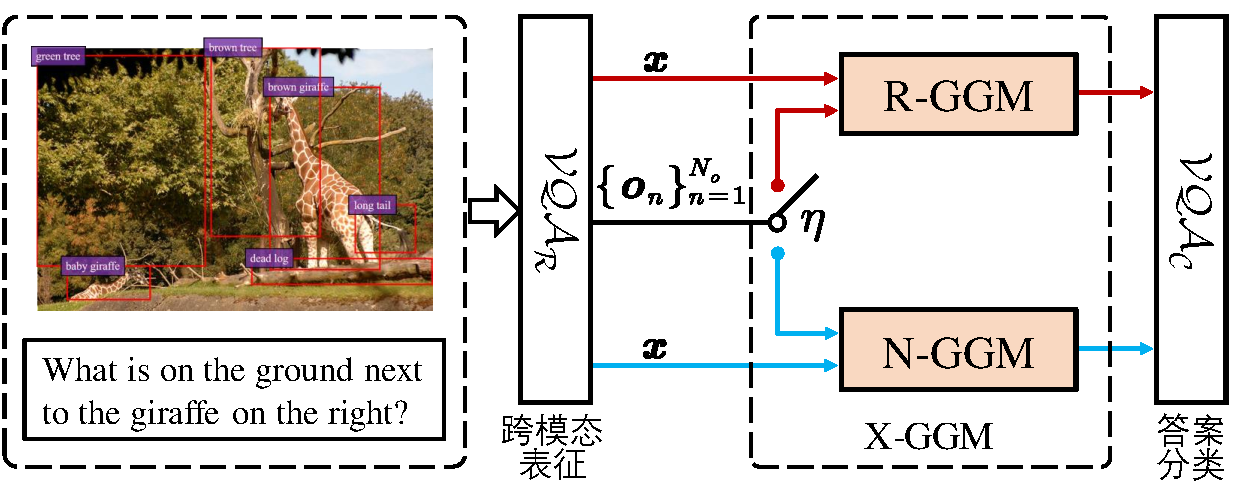
\includegraphics[width=0.8\linewidth]{figure/c3_view2.pdf}
\caption{使用X-GGM训练基线视觉问答模型的流程概述
% 。R-GGM和N-GGM是X-GGM的核心模块;$\VQAR$和$\VQAC$分别是跨模态表征模块和答案分类模块。
}
\label{fig:c3_overview} 
\end{figure}
% ********************************************************************




% **************************************************************************
\xsection{预备知识}{Preliminary} 

在本节,本章首先描述了视觉问答任务的正式定义,然后介绍了本章所使用的两种基线模型,即LXMERT~\cite{tan2019lxmert} 和UpDn~\cite{anderson2018bottom}。

\xsubsection{任务的表述}{Problem Definition}
将开放式的视觉问答任务视为多答案分类问题,视觉问答模型要求在理解相关问题$q$和图像$I$的基础上,从预定义的可能答案集($a \in \mathbb{A}$)中识别出正确答案。通常,一个视觉问答模型($\VQA$)主要包含两个模块:跨模态表征($\VQAR$)和答案分类器($\VQAC$)。数学上,该过程可以表述为
\begin{equation}
\begin{aligned}
\hat{a} = \VQAC (\xv; \thetav_{\mathcal{C}}), ~\xv = \VQAR (q, I; \thetav_{\mathcal{R}}), 
\end{aligned}
\end{equation}
式中,$\hat{a}$表示模型预测的答案,$\thetav_{\mathcal{R}}$和$\thetav_{\mathcal{C}}$分别表示跨模态表征和答案分类器的参数。$\VQAR$是核心的模块,决定了视觉问答模型的表征能力。
因此,要实现视觉问答模型分布外泛化即需要在保持$\xv$的表征能力的同时提高它的泛化能力。

\xsubsection{基线模型介绍}{Baseline}
本章采用两种典型的视觉问答模型,即LXMERT~\cite{tan2019lxmert} 和UpDn~\cite{anderson2018bottom},作为基线视觉问答模型来检验本章提出的训练策略X-GGM在分布外泛化测试时的表现。

\subsubsection{LXMERT}
LXMERT是基于跨模态预训练的经典Transformer~\cite{vaswani2017attention},由两个分别用于视觉和语言模态的单模态编码器和一个用于在两种模态之间对齐的跨模态编码器组成。LXMERT输出视觉特征序列$\{\ov_n | \ov_n \in \mathbb{R}^d, 1 \le n \le N_o \}$、语言特征序列和跨模态特征向量$\xv \in \mathbb{R}^d$;其中$N_o$表示图像帧中目标的数量,$\bm{o}_n$是$n$目标的特征向量。视觉特征序列$\{\ov_n\}$和跨模态特征向量$\xv$将被传入到X-GGM中用于提高表征$\xv$的分布外泛化能力。

\subsubsection{UpDn}
Bottom-Up Top-Down模型(UpDn)是典型的基于注意力机制的视觉问答模型。
对于图像帧$I$,UpDn首先使用图像编码器生成目标特征序列$\{\ov_n | \ov_n \in \mathbb{R}^d , 1 \le n \le N_o\}$。对给定的问题,UpDn然后使用问题编码器输出语言特征序列。
最后,获得的目标特征和语言特征被传入到一个注意力模块来生成用于答案预测的联合表征$\xv \in \mathbb{R}^d$。
而获得的$\{\ov_n\}$和$\xv$即为X-GGM的输入。


% **************************************************************************
\xsection{图生成建模}{Graph Generative Modeling} 

为了提高表征$\xv$的分布外泛化能力,考虑到在图节点信息聚合过程中自然蕴涵的组合泛化属性,本章提出了一种基于图生成建模的训练策略X-GGM。
使用X-GGM方案训练基线视觉问答模型的过程如算法~\ref{alg:c3_ggm}所示。
% ,主要包含两部分:图生成建模(X-GGM)和基线视觉问答模型更新(BMU)将会在每一次训练迭代的过程中
在$\VQAR$生成跨模态表征$\xv$和视觉特征序列$\{\ov_n | \ov_n \in \mathbb{R}^d, 1 \le n \le N_o \}$后,X-GGM以$\eta$和$1-\eta$的概率交替地利用R-GGM生成新的关系矩阵和利用N-GGM生成新的节点表征。
而在整个训练过程中,本章会先使用X-GGM策略更新一次模型参数,然后在标准范式下也更新一次模型参数,以保持视觉问答模型分布内的性能。
接下来,本节将对目标关系图的构建以及R-GGM和N-GGM进行详细介绍。


% **************************************************************************
\begin{algorithm}[!t]
\newcommand\mycommfont[1]{\footnotesize\ttfamily\textcolor{blue}{#1}}
\SetCommentSty{mycommfont}
\caption{使用X-GGM训练基线视觉问答模型}
\label{alg:c3_ggm}
\SetAlgoLined
\SetKwInput{KwInput}{Input}
\SetKwInput{KwOutput}{Output}
\DontPrintSemicolon

\KwInput{图像 $I$, 问题 $q$, 关系矩阵 $\Rmat_{GT}$}
\KwOutput{答案概率分布 $\{p_{a} | a\in \mathbb{A}\}$, 总损失 $\mathcal{L}$}

$\{\ov_n | \ov_n \in \mathbb{R}^d, 1 \le n \le N_o \}, \xv \leftarrow \VQAR(I, q)$;

\SetKwFunction{FMain}{X-GGM}
\SetKwFunction{FUpdate}{BMU}

\SetKwProg{Fn}{Function}{:}{}
\Fn{\FMain{$\ov_n, \xv$}}{
$cond \sim U[0, 1]$;\;
\eIf{$cond \leq \eta $}{  
\tcp*[l]{执行 R-GGM}
使用$\xv$和$\sigma$初始化关系矩阵$\Rmat_0$; \;
使用$\{\ov_n\}$和$\Rmat_0$进行图关系矩阵生成得到$\Rmat_g, ~\{\bar{\vv}_1, \dots, \bar{\vv}_{N_k}\}$;\;
使用$\xv$和 $\bar{\vv}_{N_k}$计算答案分布的似然估计$\{p_a\}$;\;
通过最小化R-GGM过程中的总损失$\mathcal{L}$ 更新模型参数;\;
}{
\tcp*[l]{执行 N-GGM}
使用$\xv$和$\sigma$初始化节点表征$\{\vv_i, 1\le i\le N_o \}_0$;\;
使用$\{\vv_i \}_0$ 和$\Rmat_{GT}$进行图节点表征生成得到$\Vmat_g, ~\{\bar{\vv}_1, \dots, \bar{\vv}_{N_k}\}$;\;
使用$\xv$和 $\bar{\vv}_{N_k}$计算答案分布的似然估计$\{p_a\}$;\;
通过最小化N-GGM过程中的总损失$\mathcal{L}$ 更新模型参数;\;
}
\KwRet $\{p_a\}, \mathcal{L}$\;
}
% \;
% \SetKwProg{Fn}{Function}{:}{}
% \Fn{\FUpdate{$I, q, a$}}{
% \tcp*[l]{训练基线模型}
% $\{p_a\} \leftarrow \VQA(I, q, a)$;\;
% \KwRet $\{p_a\}, \mathcal{L}$\;
% }
% % \;
\KwRet \;
\end{algorithm}
% **************************************************************************


\xsubsection{图构建}{Graph Construction}
在X-GGM中,本章以图像帧中的目标为节点构建目标关系图。
具体来说,该图可以表述为$\mathcal{G} = (\mathcal{V}, \Amat, \Rmat)$;其中$\mathcal{V} = \{v_1, \dots, v_{N_o}\}$为图顶点,$|\mathcal{V}|=N_o$为节点集合,$\Amat$是连接矩阵,$a_{i,j} \in \Amat$标记节点$v_i$和 $v_j$之间是否存在边相连,$\Rmat$是刻画节点间语义一致性的关系矩阵。构建的图$\mathcal{G}$是全连接图,即$\Amat$是全1矩阵。因此,为了简洁起见,在下文中省略$\mathcal{G}$中的$\Amat$。
在R-GGM中,为确定关系矩阵的真值$\Rmat_{GT}$,本章计算目标类别嵌入$\{\cv_n | \cv_n \in \mathbb{R}^d, 1 \le n \le N_o \}$和目标属性嵌入$\{\av_n | \av_n \in \mathbb{R}^d, 1 \le n \le N_o \}$之间余弦相似矩阵。$\cv_n$和$\av_n$由预训练后的BERT~\cite{devlin2018bert}获得。
实际上,相似度计算就是一幅图像中目标类别和目标属性的随机组合,这个过程即产生了新的组合。
在N-GGM中,本章将$\VQAR$生成的目标特征$\ov_n$作为$i$节点表征的真值,即$\vv_{GT,i} = \ov_n$。


\xsubsection{图关系的生成建模}{Graph Relation Generative Modeling}

图关系的生成建模(R-GGM)包含了三个阶段:使用$\xv$和高斯噪声初始化关系矩阵、图关系矩阵生成和R-GGM中的对抗学习。


\subsubsection{初始化关系矩阵}
图$\mathcal{G}$是具有$N_o$个节点的无向图。因此,关系矩阵$\Rmat \in \mathbb{R}^{N_o \times N_o}$是对称的,这意味着只需要初始化不包含对角元素(总为1)的上三角矩阵元素。
具体来说,本章首先使用公式~(\ref{eq:c3_trans})将$\xv$变换为向量$\rv \in \mathbb{R}^{N_o(N_o-1)/2}$。
\begin{equation}
\begin{aligned}
\rv &= \Sigmoid \left(\Wmat_{r} \xv + \bv_{r} \right), 
\label{eq:c3_trans}
\end{aligned}
\end{equation}
式中,$\Wmat_r \in \mathbb{R}^{N_o(N_o-1)/2 \times d}$为变换矩阵,可学习的偏移量$\bv_{r}$和$\rv$具有相同的维度;$\Sigmoid$表示Sigmoid激活函数。
然后,本章向$\rv$中添加标准差为$\sigma$的高斯噪声使得$\hat{\rv} \sim p_{\sigma}(\hat{\rv}|\rv)$:
\begin{equation}
\begin{aligned}
p_{\sigma}(\hat{\rv}|\rv) = \frac{1}{\sqrt{2\pi}\sigma}\exp \{-\frac{(\hat{\rv} - \rv)^2}{2\sigma^2} \}.
\label{eq:p_sigma}
\end{aligned}
\end{equation}
最后,本章用$\hat{\rv}$的元素依次填充$\Rmat_0$的上三角部分(即$\Rmat_0^{\bot}$)并通过$\Rmat_0 = \Rmat_0^{\bot} + (\Rmat_0^{\bot})^{\Transpose}$获得初始的关系矩阵。


% ********************************************************************
\begin{figure*}[!t]
\centering
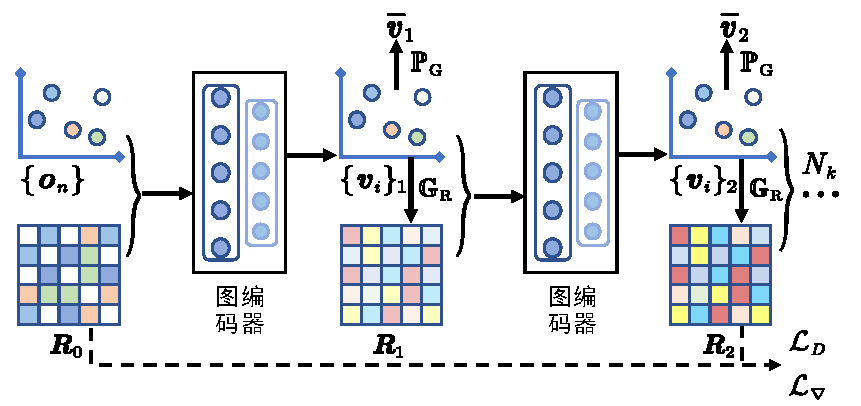
\includegraphics[width=0.85\linewidth]{figure/c3_Rel_GGM.pdf}
\caption{图关系生成}
\label{fig:c3_Rel_GGM}
\end{figure*}
% ********************************************************************



\subsubsection{图关系矩阵生成}
图关系矩阵生成的具体过程如图~\ref{fig:c3_Rel_GGM}所示,该过程可以通过$N_k$次迭代完成。
在迭代开始时,本章使用目标特征向量$\vv_{i}=\ov_{n} (i=n)$ 初始化图$\mathcal{G}$ 的节点表征。
在第$k~(1\le k \le N_k)$次迭代时,图编码器在$(k-1)$次迭代时输出的节点表征$\Vmat_{k-1} = \{\vv_i \}_{k-1}$ 和关系矩阵$\Rmat_{k-1}$ 首先被传入第$k$次迭代时的图编码器作为输入,即,$\Vmat_k^{(0)}=\Vmat_{k-1} \in \mathbb{R}^{N_o \times d}$和$\Rmat_{k}^{(0)} = \Rmat_{k-1} \in \mathbb{R}^{N_o \times N_o}$。
然后,节点表征被图编码器编码。图编码器本质上是一个具有$N_l$层的图神经网络网络。
具体来说,图编码器第$l$层中的节点表征可以通过以下方式进行节点更新:
\begin{equation}
\Vmat^{(l+1)}_k = \Sigmoid((\Rmat_{k}^{(0)}\Vmat^{(l)}_k)\Wmat^{(l)}_k + \bv^{(l)}_k), 
\end{equation}
式中,$\Wmat^l_k \in \mathbb{R}^{N_o \times d \times d}$由$N_o$个特征变换矩阵张成;$\bv_k^l \in \mathbb{R}^{N_o \times d}$是变换偏移量。
接下来,本章将R-GGM的输入和图编码器每一层的输出堆叠起来得到第$k$层的最终输出$\Vmat_{k}$:
\begin{equation}
\Vmat_{k} = \sum_{l=0}^{N_l} \ReLU(\Vmat_k^{(l)}\Wmat_a + \bv_a), 
\label{eq:Encoder_sum}
\end{equation} 
式中,$\ReLU$表示ReLU激活函数;$\Wmat_a \in \mathbb{R}^{N_o \times d \times d}$和$\bv_a \in \mathbb{R}^{N_o \times d}$是节点特征变换矩阵和偏移量。
最后,本章通过公式~(\ref{eq:c3_RG})用得到的最终节点表征$\Vmat_{k}$生成关系矩阵:
\begin{equation}
\Rmat_k = \Sigmoid(\Vmat_k\Vmat_k^{\Transpose}).
\label{eq:c3_RG}
\end{equation}
本章使用最后一次迭代的输出作为最终生成的关系矩阵,即,$\Rmat_g = \Rmat_{N_k}$。此外,本章对节点表征$\{\vv_i, 1\le i \le N_o\}_{k}$计算平均值作为第$k$次迭代的图表征$\bar{\vv}_{k}$。


% ********************************************************************
\begin{figure*}[!t]
\centering
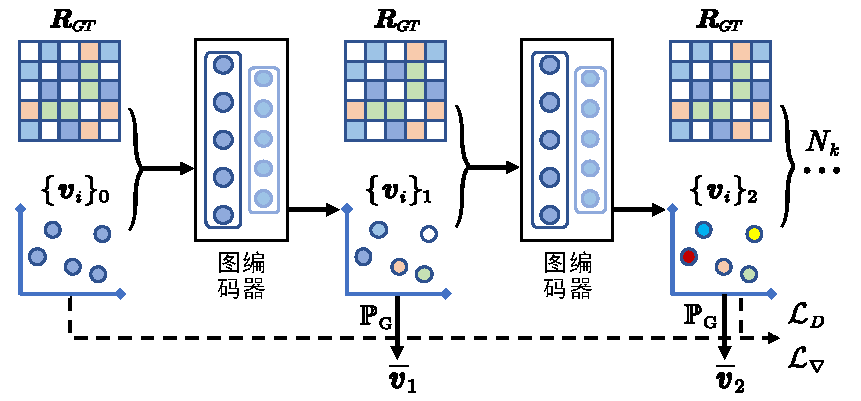
\includegraphics[width=0.85\linewidth]{figure/c3_Rep_GGM.pdf}
\caption{图表征生成}
\label{fig:c3_Rep_GGM}
\end{figure*}
% ********************************************************************

\subsubsection{R-GGM中的对抗学习}
在初始化关系矩阵时,本章发现R-GGM引入对抗性扰动的过程与去噪自编码~\cite{vincent2008extracting} 的过程十分相似。
从最近的研究~\cite{bigdeli2020learning} 中本章知道,对于加性白高斯噪声的最佳去噪自编码器可以显式地计算出来且与加入噪声后的数据分布梯度有关。
实际上,添加了对抗性扰动的数据分布的对数梯度可以用公式~(\ref{eq:p_sigma})导出,如下:
\begin{equation}
\nabla_{\hat{\rv}}\log p_{\sigma}(\hat{\rv}|\rv) = -\frac{(\hat{\rv} - \rv)^2}{\sigma^2}. 
\end{equation} 
在获得$\nabla_{\hat{\rv}}\log p_{\sigma}(\hat{\rv}|\rv)$后,为了约束生成的关系矩阵$\Rmat_g$和预计算的相似矩阵$\Rmat_{GT}$之间的梯度分布一致性,本章计算生成的关系矩阵元素的对数似然梯度值$\nabla_{\rv}\log p_g(\rv)$。因此,梯度分布一致性损失可以定义为
\begin{equation} 
\mathcal{L}_{\nabla} \triangleq  \mathbb{E}\left[\left\| \nabla_{\rv}\log p_g(\rv) - \nabla_{\hat{\rv}}\log p_{\sigma}(\hat{\rv}|\rv) \right\|_2^2\right]. 
\label{eq:L_G}
\end{equation} 
除了约束梯度分布一致性,本章进一步利用KL散度来度量生成的分布$p_g(\rv)$和原始数据分布$p_{data}(\rv)$之间的距离,其中$p_g$和$p_{data}$分别表示矩阵$\Rmat_g$和$\Rmat_{GT}$ 中元素的概率分布。则,训练R-GGM的距离度量损失可以表示为
\begin{equation}
\mathcal{L}_D = \mathrm{KL}(p_g \| p_{data}) + \mathrm{KL}(p_{data} \| p_g), 
\label{eq:L_D}
\end{equation}
式中,$\mathrm{KL}(p\|q)=\mathbb{E}_{\rv \sim p}\left[\log p(\rv) - \log q(\rv)\right]$。
除了对抗损失($\mathcal{L}_{\nabla}$和$\mathcal{L}_{D}$),本章将池化后的图表征$\bar{\vv}_{N_k}$加到原始的跨模态表征$\xv$中后传入到$\VQAC$中,计算答案分布的似然估计$p_{a}$和视觉问答任务相关的BCE损失$\mathcal{L}_{\textsc{bec}}$。
综上,训练R-GGM的总损失可以表述为
\begin{equation}
\mathcal{L} = \alpha \mathcal{L}_{\nabla} + \beta \mathcal{L}_D + \mathcal{L}_{\textsc{bce}}, 
\label{eq:c3_L_total}
\end{equation} 
式中,$\alpha$和$\beta$为权重系数。


\xsubsection{图表征的生成建模}{Graph Representation Generative Modeling}

图表征的生成建模(N-GGM)过程与图关系的生成建模过程相似,也包含了三个阶段:使用$\xv$和高斯噪声初始化节点表征、节点表征生成和N-GGM中的对抗学习。

\subsubsection{初始化节点表征}
为获得图$\mathcal{G}$的$N_o$个初始节点表征,本章首先将$\xv$张成$[\xv, \dots, \xv] \in \mathbb{R}^{N_o\times d}$,并使用一个全连接层($\mathcal{M}_{\text{FC}}$)对其进行特征变换来增加初始节点表征间的差异性:
\begin{equation}
\begin{aligned}
\Vmat_{\xv} &= \mathcal{M}_{\text{FC}} ([\xv, \dots, \xv]), \Vmat_{\xv} \in \mathbb{R}^{N_o\times d},  
\end{aligned}
\end{equation}
式中,$\Vmat_{\xv}=\{\vv_{i,\xv} | \vv_{i,\xv} \in \mathbb{R}^{d}, 1\le i\le N_o \}$。
然后,本章将对抗扰动添加到$\Vmat_{\xv}$中,使得$\Vmat_{\xv}$的第$i$个特征向量$\hat{\vv}_{i, \xv}$满足噪声先验分布$p_{\sigma}(\hat{\vv}_{i, \xv} | \vv_{i, \xv})$:
\begin{equation}
\begin{aligned}
p_{\sigma}(\hat{\vv}_{i, \xv} | \vv_{i, \xv}) = \frac{1}{\sqrt{2\pi}\sigma}\exp \{-\frac{(\hat{\vv}_{i, \xv} - \vv_{i, \xv})^2}{2\sigma^2} \}. 
\end{aligned}
\end{equation}
最后,图$\mathcal{G}$的初始节点表征可以由$\Vmat_0 = \hat{\Vmat}_{\xv} = [\hat{\vv}_{0,\xv}, \dots, \hat{\vv}_{N_o,\xv}]$获得。


\subsubsection{节点表征生成}
节点表征生成的具体过程如图~\ref{fig:c3_Rep_GGM}所示。在第$k$次迭代时,图编码器在$(k-1)$次迭代时输出的节点表征$\Vmat_{k-1}= \{\vv_i, 1 \le i \le N_o \}_{k-1}$ 和预定义的关系矩阵真值$\Rmat_{GT}$首先被传入到第$k$次迭代中的图编码器中进行节点的更新。
然后,本章利用公式~(\ref{eq:Encoder_sum})生成第$k$次迭代中的图编码器的最终输出$\Vmat_k$。N-GGM中的图编码器的结构与R-GGM中相同,均为$N_l$层的图卷积网络。
本章使用最后一次迭代生成的节点表征作为N-GGM最终生成的节点表征,即,$\Vmat_g = \Vmat_{N_k}$。此外,在每次迭代时,本章平均$N_o$个节点表征$\Vmat_{k}= \{\vv_i, 1 \le i \le N_o \}_{k}$来生成图表征$\bar{\vv}_k$。




\subsubsection{N-GGM中的对抗学习}
训练N-GGM的总损失$\mathcal{L}$也是损失$\mathcal{L}_{\nabla}$、$\mathcal{L}_D$和 $\mathcal{L}_{\textsc{bce}}$的加权和。
具体来说,梯度分布一致性损失$\mathcal{L}_{\nabla}$定义为加入高斯噪声后的初始节点表征$\hat{\Vmat}_{\xv}$的分布梯度与生成的节点表征$\Vmat_g$的似然估计之间的测度。
梯度分布一致性损失可以定义为
\begin{equation} 
\mathcal{L}_{\nabla} \triangleq  \mathbb{E}\left[\left\| \nabla_{\vv_{\xv}}\log p_g(\vv_{\xv}) - \nabla_{\hat{\vv}_{\xv}}\log p_{\sigma}(\hat{\vv}_{\xv} | \vv_{\xv})  \right\|_2^2\right]. 
\label{eq:L_G2}
\end{equation} 
$\mathcal{L}_D$是生成的节点表征$\Vmat_g$的分布与$\VQAR$输出的原始节点表征$\{\ov_n\}$的分布之间的KL散度。$\mathcal{L}_{\textsc{bce}}$是视觉问答的分类损失。
综上,训练N-GGM的总损失同公式~(\ref{eq:c3_L_total})。


% **************************************************************************
\xsection{实验及结果分析}{Experiment and Result Analysis}

% **************************************************************************
\xsubsection{实验设置}{Experimental Setting}

\subsubsection{数据集}
本章在两个视觉问答分布外泛化评测数据集VQA-CP v2~\cite{agrawal2018don} 和GQA-OOD~\cite{kervadec2021roses} 上进行了实验。
具体来说,\textbf{VQA-CP v2}是对VQA v2~\cite{shih2016look}训练集和验证集的重新组织。
为了评估视觉问答模型的分布外泛化能力,Agrawal 等人~\cite{agrawal2018don} 通过使每种类型的问题的答案在训练集和测试集上分布不同构建了VQA-CP v2数据集。原始的VQA-CP v2仅包含训练集和测试集,即没有官方的验证集。因此,为了给VQA-CP v2创建验证集,本章对数据集进行了重新划分,重划分后的数据集的统计信息如表~\ref{tab:c3_dataset}所示。
\textbf{GQA-OOD}是对GQA~\cite{hudson2019gqa}数据集的细化重组,通过在GQA的验证集和测试集中引入答案分布偏移来获得GQA-OOD的验证集和测试集。但GQA-OOD具有和GQA相同的训练集。统计信息如表~\ref{tab:c3_dataset}所示。
此外,GQA-OOD提供了四种评价指标:(\emph{i}) \textbf{Tail}:在分布外测试样本上的VQA-Score;(\emph{ii}) \textbf{Head}:在域内测试样本上的VQA-Score; (\emph{iii}) \textbf{All}:在所有测试样本上的VQA-Score; (\emph{iv}) $\Delta (\%)\textup{ = (head - tail) / tail}$: 度量视觉问答模型预测的错误答案在高频和罕见答案之间的不平衡程度。


\begin{table}[!t]
\caption{数据集的统计信息}
\label{tab:c3_dataset}
\setlength{\tabcolsep}{0.7mm}{
\begin{tabularx}{\textwidth}{@{}lcccccccccc@{}}
\toprule
\multirow{2}{*}{Dataset}  
&\multicolumn{5}{c}{Image} 
&\multicolumn{5}{c}{Question} 
% &\multirow{2}{*}{Year} 
\\

\cmidrule(lr){2-6}
\cmidrule(l){7-11}
&Train &Val &OOD &ID &Total
&Train &Val &OOD &ID &Total
% & 
\\ 
\midrule

VQA-CP v2~\cite{agrawal2018don}
& \eqmakebox[log][r]{119,107} & \eqmakebox[log][r]{31,976} 
& \eqmakebox[log][r]{89,437} & \eqmakebox[log][r]{32,266} 
& \eqmakebox[log][r]{272,786} 
& \eqmakebox[log][r]{388,735} & \eqmakebox[log][r]{38,802}
& \eqmakebox[log][r]{179,928} & \eqmakebox[log][r]{40,000} 
& \eqmakebox[log][r]{647,465} 
% &2018 
\\

GQA-OOD~\cite{kervadec2021roses} 
& \eqmakebox[log][r]{72,140} & \eqmakebox[log][r]{9,406} 
& \eqmakebox[log][r]{330} & \eqmakebox[log][r]{365} 
& \eqmakebox[log][r]{82,241} 
& \eqmakebox[log][r]{943,000} & \eqmakebox[log][r]{51,045} 
& \eqmakebox[log][r]{1,063} & \eqmakebox[log][r]{1,733} 
& \eqmakebox[log][r]{996,841} 
% &2020 
\\ 
\bottomrule
\end{tabularx}
}
\end{table}


\subsubsection{评价指标}
考虑到通常情况下一个问题对应的正确答案并不是唯一的,本章遵循Antol等人~\cite{antol2015vqa} 对视觉问答模型性能的评测,以VQA-Score为视觉问答性能的评价指标。即,
% 本文在VQA-CP v2和GQA-OOD数据集上的评价指标如下:
\begin{equation}
\begin{aligned}
\text{VQA-Score} (a) = \min \{\frac{C_a}{3}, 1\}, ~a \in \mathbb{A},  
\end{aligned}
\end{equation} 
式中,$C_a$表示模型预测的答案$a$出现在该问题对应的正确答案集合中的次数,当$C_a \ge 3$时则认为$a$为正确答案。


\subsubsection{数据预处理细节}
Teney 等人~\cite{teney2020value}的相关研究表明在VQA-CP v2数据集上评价视觉问答模型的分布外性能存在一些不足之处,特别是使用分布外数据的测试集进行模型选择和在VQA v2上重新训练视觉问答模型后评价视觉问答模型的域内性能。
因此,按照最近的相关工作~\cite{teney2019actively,teney2020unshuffling,teney2020learning,clark2020learning},本章重新划分了VQA-CP v2。
具体来说,本章从训练集中保留40k个随机样本来评估视觉问答模型的域内性能,并从分布外测试集中保留40k个随机样本用于模型选择。
此外,本章使用在VG~\cite{krishna2017visual} 数据收集上预训练后的BUA Faster R-CNN~\cite{anderson2018bottom} 提取图像帧中目标的类别和属性。


\subsubsection{实现细节}
对于本章提出的X-GGM,本章设置图$\mathcal{G}$中节点的个数$N_o$为36,标准特征维度$d$为768。公式~(\ref{eq:p_sigma})中的标准差$\sigma$为1.0。算法~\ref{alg:c3_ggm}中阈值$\eta$在VQA-CP v2和GQA-OOD数据集上分别为0.8和0.5。使用X-GGM训练时总的迭代次数$N_k$为2。图编码器的层数$N_l$为2。公式~(\ref{eq:c3_L_total})中的权重系数$\alpha$和$\beta$在R-GGM时为6和72,在N-GGM时为6.6和0.17。
本章利用PyTorch深度学习框架,在一张NVIDIA GTX2080 12GB GPU上进行了实验。在训练过程中,本章使用AdamW~\cite{loshchilov2017decoupled}优化器,训练轮次为5、初始学习率为$1\times 10^{-6}$、批大小为128。



% **************************************************************************
\xsubsection{与不同方法的性能比较}{Comparison with State-of-the-Arts}

为了评估用X-GGM训练基线视觉问答模型的分布外和域内性能,本章在VQA-CP v2和GQA-OOD数据集上与当时已有的方法进行了比较。

\begin{table}[!t]
\caption{在VQA-CP v2数据集上的性能 (\%) 比较
% 。$^{\dagger}$:该方法使用了额外人工标注的数据;$^{*}$:我们使用开源代码重新实现的结果;--:该方法未评测相关性能。
}
\label{tab:c3_vqacpv2}
\setlength{\tabcolsep}{2.79mm}{
\begin{tabularx}{\textwidth}{@{}lcccccccc}
\toprule
\multirow{2}{*}{Method} 
&\multicolumn{4}{c}{VQA-CP v2 OOD Test} 
% \textcolor{blue}{$\uparrow$}
&\multicolumn{4}{c}{VQA-CP v2 ID Test} 
% \textcolor{blue}{$\uparrow$}
\\ 

\cmidrule(lr){2-5}
\cmidrule(l){6-9}
&All &Yes/No &Num. &Other 
&All &Yes/No &Num. &Other 
\\ 
\midrule

% *********************************************************************
\multicolumn{9}{c}{\textbf{KB-based Method}} 
\\
RankVQA~\cite{qiao2020rankvqa} 
&43.05 &42.53 &13.19 &\cellcolor{cyan!10}{51.32} 
&-- &-- &-- &\cellcolor{cyan!10}{--} 
\\

% LM~\cite{clark2019don} 
% &48.78 &72.78 &14.61 &\cellcolor{cyan!10}{45.58} 
% &-- &-- &-- &\cellcolor{cyan!10}{--} 
% \\

LMH~\cite{clark2019don} 
&52.01 &72.58 &31.12 &\cellcolor{cyan!10}{46.97} 
&-- &-- &-- &\cellcolor{cyan!10}{--} 
\\
\, + LRS~\cite{guo2021loss} 
&53.26 &72.82 &48.00 &\cellcolor{cyan!10}{44.46}
&-- &-- &-- &\cellcolor{cyan!10}{--} 
\\
\, + CCB+VQ-CSS~\cite{yang2021learning} 
&59.12 &89.12 &51.04 &\cellcolor{cyan!10}{45.62} 
&-- &-- &-- &\cellcolor{cyan!10}{--} 
\\
\, + MFE~\cite{gat2020removing} 
&54.55 &74.03 &49.16 &\cellcolor{cyan!10}{45.82} 
&-- &-- &-- &\cellcolor{cyan!10}{--} 
\\
\, + CSS+CL~\cite{liang2020learning} 
&59.18 &86.99 &49.89 &\cellcolor{cyan!10}{47.16} 
&-- &-- &-- &\cellcolor{cyan!10}{--} 
\\

\, + CSS+GS~\cite{liang2020learning}
&57.37 &79.71 &50.85 &\cellcolor{cyan!10}{47.45} 
&-- &-- &-- &\cellcolor{cyan!10}{--} 
\\

\, + CSS~\cite{chen2020counterfactual} 
&58.95 &84.37 &49.42 &\cellcolor{cyan!10}{48.21} 
&-- &-- &-- &\cellcolor{cyan!10}{--} 
\\ 
\, + CCB~\cite{yang2021learning} 
&57.99 &86.41 &45.63 &\cellcolor{cyan!10}{48.76} 
&-- &-- &-- &\cellcolor{cyan!10}{--} 
\\

\midrule[0.5pt]
\midrule[0.5pt]
% *********************************************************************
\multicolumn{9}{c}{\textbf{UB-based Method}} 
\\
GVQA~\cite{agrawal2018don} 
&31.30 &57.99 &13.68 &\cellcolor{cyan!10}{22.14}
&-- &-- &-- &\cellcolor{cyan!10}{}{--} 
\\
Actively Seeking~\cite{teney2019actively} 
&46.00 &58.24 &29.49 &\cellcolor{cyan!10}{44.33} 
&-- &-- &-- &\cellcolor{cyan!10}{--} 
\\
VGQE~\cite{kv2020reducing} 
&50.11 &66.35 &27.08 &\cellcolor{cyan!10}{46.77} 
&-- &-- &-- &\cellcolor{cyan!10}{--} 
\\

Unshuffling~\cite{teney2020unshuffling} 
&42.39 &47.72 &14.43 &\cellcolor{cyan!10}{47.24} 
&-- &-- &-- &\cellcolor{cyan!10}{--} 
\\

Unshuffling+CF~\cite{teney2020learning} 
&40.60 &61.30 &15.60 &\cellcolor{cyan!10}{46.00} 
&63.30 &79.40 &45.50 &\cellcolor{cyan!10}{53.70} 
\\

Unshuffling+CF+GS~\cite{teney2020learning}
&46.80 &64.50 &15.30 &\cellcolor{cyan!10}{45.90}
&62.40 &77.80 &43.80 &\cellcolor{cyan!10}{53.60}
\\ 

% *********************************************************************
% \cmidrule(lr){2-9}
\midrule
UpDn~\cite{anderson2018bottom} 
&38.82  &42.98  &12.18  &\cellcolor{cyan!10}{43.95} 
&64.73  &79.45  &49.59  &\cellcolor{cyan!10}{55.66}  
\\

\, + Top answer masked~\cite{teney2020value} 
&40.61  &82.44  &27.63  &\cellcolor{cyan!10}{22.26} 
&30.90  &44.12  &5.00  &\cellcolor{cyan!10}{20.85} 
\\ 
\, + AdvReg~\cite{grand2019adversarial} 
&36.33  &59.33  &14.01  &\cellcolor{cyan!10}{30.41} 
&50.63  &67.39  &38.81  &\cellcolor{cyan!10}{38.37} 
\\ 
\, + GRL~\cite{grand2019adversarial}
&42.33 &59.74 &14.78 &\cellcolor{cyan!10}{40.76} 
&56.90 &69.23 &42.50 &\cellcolor{cyan!10}{49.36} 
\\

\, + RUBi~\cite{cadene2019rubi} 
&47.11 &68.65 &20.28 &\cellcolor{cyan!10}{43.18} 
&-- &-- &-- &\cellcolor{cyan!10}{--} 
\\

\, + RandImg ($\lambda$=12)~\cite{teney2020value} 
&55.37  &83.89  &41.60  &\cellcolor{cyan!10}{44.20}  
&54.24  &64.22  &34.40  &\cellcolor{cyan!10}{50.46}
\\
\, + RandImg ($\lambda$=5)~\cite{teney2020value}
&51.15  &75.06  &24.30  &\cellcolor{cyan!10}{45.99}  
&59.28  &70.66  &43.06  &\cellcolor{cyan!10}{53.40} 
\\ 

\, + CF-VQA (Sum)~\cite{niu2021counterfactual}
&53.69 &91.25 &12.80 &\cellcolor{cyan!10}{45.23} 
&-- &-- &-- &\cellcolor{cyan!10}{--}  
\\

\, + CF-VQA (Har.)~\cite{niu2021counterfactual}
&49.94 &74.82 &18.93 &\cellcolor{cyan!10}{45.42} 
&-- &-- &-- &\cellcolor{cyan!10}{--}  
\\

\, + DLR~\cite{jing2020overcoming} 
&48.87 &70.99 &18.72 &\cellcolor{cyan!10}{45.57}  
&-- &-- &-- &\cellcolor{cyan!10}{--} 
\\

\, + HINT(HAT)$^{\dagger}$~\cite{selvaraju2019taking} 
&47.70 &70.04 &10.68 &\cellcolor{cyan!10}{46.31} 
&-- &-- &-- &\cellcolor{cyan!10}{--} 
\\

\, + SCR (HAT)$^{\dagger}$~\cite{wu2019self} 
&49.17 &71.55 &10.72 &\cellcolor{cyan!10}{47.49} 
&-- &-- &-- &\cellcolor{cyan!10}{--} 
\\

\, + SCR (VQA-X)$^{\dagger}$~\cite{wu2019self} 
&49.45 &72.36 &10.93 &\cellcolor{cyan!10}{48.02} 
&-- &-- &-- &\cellcolor{cyan!10}{--} 
\\

\, + SL~\cite{zhu2020overcoming} 
&57.59 &86.53 &29.87 &\cellcolor{cyan!10}{50.03}  
&-- &-- &-- &\cellcolor{cyan!10}{--} 
\\

\, + MUTANT$^{\dagger}$~\cite{gokhale2020mutant}
&61.72 &88.90 &49.68 &\cellcolor{cyan!10}{50.78} 
&-- &-- &-- &\cellcolor{cyan!10}{--} 
\\

\, \textbf{+ X-GGM} 
&45.71  &43.48  &27.65  &\cellcolor{cyan!10}{{52.34}}   
&67.16  &83.74  &48.26  &\cellcolor{cyan!10}{{56.91}} 
\\ 

% \cmidrule(lr){2-9}
% *********************************************************************
\midrule
LXMERT$^{*}$~\cite{tan2019lxmert} 
&63.90 &80.45 &46.58 &\cellcolor{cyan!10}{{59.98}} 
&75.57 &91.39 &59.83 &\cellcolor{cyan!10}{65.21}
\\

\, + MUTANT$^{\dagger}$~\cite{gokhale2020mutant}
&{69.52} &93.15 &67.17 &\cellcolor{cyan!10}{57.78} 
&- &- &- &\cellcolor{cyan!10}{-} 
\\

\, + VILLA$^*$~\cite{gan2020large} 
&48.06 &42.66 &18.97 &\cellcolor{cyan!10}{58.89} 
&{75.85} &90.40 &60.02 &\cellcolor{cyan!10}{{66.66}} 
\\

\, + MCE+Adv~\cite{clark2020learning} 
&66.08 &-- &-- &\cellcolor{cyan!10}{--}
&{\text{77.17}} &-- &-- &\cellcolor{cyan!10}{--}
\\

\, + MCE~\cite{clark2020learning} 
&{68.44} &-- &-- &\cellcolor{cyan!10}{--}
&74.03 &-- &-- &\cellcolor{cyan!10}{--}
\\

\, \textbf{+ X-GGM} 
&66.95 &78.91 &53.63 &\cellcolor{cyan!10}{{\textbf{64.33}}} 
&75.88 &90.18 &60.06 &\cellcolor{cyan!10}{{\textbf{66.92}}} 
\\
\bottomrule
\end{tabularx}
}
\end{table}


\subsubsection{在VQA-CP v2数据集上的实验}
X-GGM是一种在保持域内性能的同时提高基线视觉问答模型分布外泛化能力的训练策略。
它在一定程度上减小了视觉问答模型的语言偏见,而无需事先知道偏见。
因此,根据视觉问答去偏方法是否需要事先知道数据中的偏见,本章将已有的方法分为两类。
(\emph{i}) 基于已知偏见的方法(\text{KB-based}): LMH~\cite{clark2019don}、LRS~\cite{guo2021loss} 和LMH-MFE~\cite{gat2020removing}。
(\emph{ii}) 基于未知偏见的方法(\text{UB-based}): MCE~\cite{clark2020learning}、MUTANT~\cite{gokhale2020mutant}、Unshuffling~\cite{teney2020unshuffling} 和VILLA~\cite{gan2020large}。
特别是,VILLA~\cite{gan2020large} 采用将噪声引入表征空间的对抗训练策略来提高模型的泛化能力。这种将对抗性扰动引入表征空间的策略启发了本章的工作。
因此,本章在VQA-CP v2上重新实现了 VILLA,以便进行更公平的比较。
在VQA-CP v2上,本章使用LXMERT和UpDn作为基线视觉问答模型,主要将提出的X-GGM方案与基于未知偏见的方法进行比较。
虽然本章在 VQA-CP v2 ``All''上进行了实验,但将实验结果比较重点放在``Other''上而不是``Yes/No''和 ``Num''上,因为``Other''类型的问题可以更好地评估视觉问答模型分布外的泛化能力。 
实验结果如表~\ref{tab:c3_vqacpv2}所示。使用本章节提出的X-GGM方案训练,基线视觉问答模型(LXMERT)在VQA-CP v2 ``Other''上取得了最优的分布外和域内性能。
此外,与所有使用UpDn作为基线视觉问答模型的方法相比,本章的方法在“Other”上也获得了最好的分布外和域内性能。
这些结果均表明,X-GGM方案在保持视觉问答模型域内性能的同时能有效地将模型泛化到分布外的样本。



\begin{table}[!t]
\caption{在GQA-OOD数据集上的性能比较
% \textcolor{blue}{$\uparrow$} (\textcolor{red}{$\downarrow$}) 表示值越高(低)越好。
}
\label{tab:c3_gqa_ood}
\setlength{\tabcolsep}{10.8mm}{
\begin{tabularx}{\textwidth}{@{}lcccc@{}}
\toprule
\multirow{2}{*}{Method}
&\multicolumn{4}{c}{Metrics (\%)} 
\\

\cmidrule(l){2-5}

&All \textcolor{blue}{$\uparrow$}
&\text{Tail} \textcolor{blue}{$\uparrow$}
&Head \textcolor{blue}{$\uparrow$}
&$\Delta$ \textcolor{red}{$\downarrow$} 
\\ 
\midrule
\multicolumn{5}{c}{\textbf{Plain Model}} 
\\
% 结果来自于GQA-OOD benchmark 提出的文章
BAN4~\cite{kim2018bilinear} &50.20 
&{47.20} &51.90 &9.90 \\ 
% meta module network
MMN~\cite{chen2021meta} &52.70 
&{48.00} &55.50 &15.60 \\ 
UpDn~\cite{anderson2018bottom} &46.40 
&{42.10} &49.10 &16.60 \\
\, + LMH~\cite{clark2019don} &33.10 
&{30.80} &34.50 &12.00 \\
\, + LM~\cite{clark2019don} &34.50 
&{32.20} &35.90 &11.50 \\ 

\, + RUBi~\cite{cadene2019rubi} &38.80 
&{35.70} &40.80 &14.30 \\

\, \textbf{+ X-GGM} &48.41 
&{45.99} &{49.90} &\textbf{8.51} 
\\

\midrule

\multicolumn{5}{c}{\textbf{Transformer-based Model}} 
\\
MCAN~\cite{yu2019deep} &50.80 
&{46.50} &53.40 &14.80 
\\  % transformer 
MANGO (UNITER)~\cite{li2020closer} &\textbf{56.40} 
&51.27 &\textbf{59.55} &16.15 
\\ 
LXMERT~\cite{tan2019lxmert}
&54.60 &{49.80} &\text{57.70} &15.90 
\\ 
\, + VILLA$^{*}$~\cite{gan2020large} 
&54.47 
&{49.95} &57.24 &14.59 
\\
\, + MANGO~\cite{li2020closer} 
&54.94 &{--} &-- &-- 
\\

\, \textbf{+ X-GGM} 
&\text{55.59} 
&{\textbf{52.47}} &57.51 &\text{9.59} 
\\ 
\bottomrule
\end{tabularx}    
}
\end{table}
\subsubsection{在GQA-OOD数据集上的实验}
在GQA-OOD数据集上评测的所有对比方法中,除LMH~\cite{clark2019don}和LM~\cite{clark2019don} 外,其它的方法都是于未知偏见的。这类基于未知偏见的方法可以进一步分为:(\emph{i}) 传统模型(Plain Model): BAN4~\cite{kim2018bilinear}、MMN~\cite{chen2021meta}、UpDn~\cite{anderson2018bottom}、LMH~\cite{clark2019don}、LM~\cite{clark2019don} 和RUBi~\cite{cadene2019rubi};(\emph{ii}) 基于Transformer的模型(Transformer-based Model): MCAN~\cite{yu2019deep}、LXMERT~\cite{tan2019lxmert}、VILLA~\cite{gan2020large} 和MANGO~\cite{li2020closer}。
X-GGM使用LXMERT和UpDn作为基线视觉问答模型,RUBi、LMH和LM使用UpDn为基线视觉问答模型,而VILLA和MANGO使用LXMERT为基线视觉问答模型。
本章在GQA-OOD数据集上重新实现了VILLA。
从表~\ref{tab:c3_gqa_ood} 中的实验结果中本章可以观察到,使用本章提出的X-GGM训练的基线视觉问答模型(LXMERT)在度量~\textbf{Tail} 上优于GQA-OOD上的其他方法。虽然域内性能(Head)相对于基线视觉问答模型下降了0.19,但这远小于OOD性能提升(2.67)。
此外,用X-GGM方案训练的基线视觉问答模型(UpDn)在所有指标上也优于使用UpDn作为基线视觉问答模型的方法,特别是在~\textbf{Tail}指标上。
这些结果均证明了X-GGM的分布外泛化能力。
遗憾地是在GQA-OOD上的分布外泛化性能改进并不像VQA-CP v2上的那样显著。
这可能是因为GQA-OOD数据集上的问题具有语义组合性。语法复杂的问题削弱了$\xv$的表征能力,而X-GGM也没有明确利用问题的结构化表示来增强$\xv$。



\begin{table}[!t]
\caption{关于使用$\mathcal{L}_D$和$\mathcal{L}_{\nabla}$的不同损失组合训练R-GGM和N-GGM的消融实验
% 。 \textcolor{blue}{$\uparrow$} (\textcolor{red}{$\downarrow$}) 表示值越高(低)越好。
}
\label{tab:c3_abl_comps}
\setlength{\tabcolsep}{3.24mm}{
\begin{tabularx}{\textwidth}{ccccccccccc}
\toprule
\multirow{2}{*}{S/N}
&\multicolumn{2}{c}{R-GGM}
&\multicolumn{2}{c}{N-GGM} 
&\multicolumn{3}{c}{VQA-CP v2 ``Other'' (\%)}
&\multicolumn{3}{c}{GQA-OOD (\%)} 
\\
\cmidrule(lr){2-3}
\cmidrule(lr){4-5}
\cmidrule(lr){6-8}
\cmidrule(l){9-11}

&\small $\mathcal{L}_{\nabla}$ 
&\small $\mathcal{L}_D$ 
&\small $\mathcal{L}_{\nabla}$
&\small $\mathcal{L}_D$ 
&\small OOD\textcolor{blue}{$\uparrow$}
&\small ID\textcolor{blue}{$\uparrow$}
&\small Gap\textcolor{red}{$\downarrow$} 
&\small Tail\textcolor{blue}{$\uparrow$} 
&\small Head\textcolor{blue}{$\uparrow$} 
&$\Delta$\textcolor{red}{$\downarrow$}
\\
\midrule
\rowcolor{gray!15}LXMERT
&\multicolumn{4}{c}{---} 
&59.98 &65.21 &5.23 
&49.80 &57.70 &15.90 \\ 
% \hline 
\#1 &\checkmark &\checkmark & & 
&63.84 &66.41 &2.57 
&51.39 &56.93 &10.77 
\\
\#2 & & &\checkmark &\checkmark 
&62.90 &65.57 &2.67
&51.27 &57.30 &11.76
\\
% \hline 
\#3 &\checkmark & &\checkmark & 
&63.75 &66.03 &\textbf{2.28} 
&51.65 &57.13 &10.61 
\\ 
\#4 & &\checkmark & &\checkmark 
&62.73 &65.99 &3.26 
&51.27 &57.19 &11.54 
\\
% \hline 
\#5 &\checkmark &\checkmark &\checkmark &\checkmark 
&\textbf{64.33} &\textbf{66.92} &2.59 
&\textbf{52.47} &\textbf{57.51} &\textbf{9.59} 
\\
\bottomrule
\end{tabularx}
} % scale box
\end{table}
% *********************************************************************

% **************************************************************************
\xsubsection{消融实验}{Ablation Study}

本章使用LXMERT为基线视觉问答模型在VQA-CP v2和GQA-OOD数据集上进行了消融实验。
考虑到相关工作~\cite{teney2020value}中的发现,即,在VQA-CP v2数据集上答案为yes、no和number的问题在评价视觉问答模型分布外的泛化能力时容易误导模型,本章主要分析模型在VQA-CP v2 ``other''上的性能。
此外,为了对比更加公平,本章在VQA-CP v2 ``All''上训练模型但在VQA-CP v2 ``other''上选择最佳模型。


\subsubsection{X-GGM核心部件的有效性}
要提高$\VQAR$生成的跨模态表征$\xv$的分布外泛化能力,除了使用完整的X-GGM策略训练基线视觉问答模型外,R-GGM或N-GGM也能单独工作。
因此,本章首先考虑X-GGM、R-GGM和N-GGM与基线视觉问答模型LXMERT的对比(即,\#1, \#2, \#5 vs. LXMERT)来分析它们各自的有效性。
具体来说,$\blacktriangleright$ LXMERT vs. \#1 (仅使用R-GGM训练基线视觉问答模型)。
$\blacktriangleright$ LXMERT vs. \#2 (仅使用N-GGM训练基线视觉问答模型)。
$\blacktriangleright$ LXMERT vs. \#5 (使用X-GGM训练基线视觉问答模型,X-GGM即以概率$\eta$和1-$\eta$交替执行R-GGM和N-GGM)。
表~\ref{tab:c3_abl_comps} 展示了在VQA-CP v2 ``Other''和GQA-OOD数据集上的实验结果。
表中\#5 / \#1 / \#2 vs. LXMERT的对比表明X-GGM、R-GGM和N-GGM均能有效地提高基线视觉问答模型的分布外泛化能力。

然后,为了探索R-GGM和N-GGM对X-GGM的重要性,本章考虑以下两组对比:
$\blacktriangleright$ 表~\ref{tab:c3_abl_comps} \#1 vs. \#5和$\blacktriangleright$ 表~\ref{tab:c3_abl_comps} \#2 vs. \#5。表中的实验结果表明R-GGM较N-GGM在提升视觉问答基线模型分布外泛化性能上更有效。这主要是因为N-GGM中因噪声引入引起的梯度不稳定性要比R-GGM中大。具体来说,添加到R-GGM和N-GGM中的噪声向量的维度分别为$N_o (N_o - 1)/2 = 630$和$N_o \times d = 27,648$。

最后,为了评估梯度分布一致性损失$\mathcal{L}_{\nabla}$在缓解不稳定梯度问题方面的有效性,本章分析了$\mathcal{L}_{\nabla}$和$\mathcal{L}_D$各自的影响。实验设置和结果如表~\ref{tab:c3_abl_comps} (\#3, \#4, \#5)所示。具体来说,\#3:在用X-GGM训练基线视觉问答模型时,仅使用$\mathcal{L}_D$作为对抗损失; \#4:在用X-GGM训练基线视觉问答模型时,仅使用$\mathcal{L}_{\nabla}$作为对抗损失; \#5:在用X-GGM训练基线视觉问答模型时,使用$\mathcal{L}_{\nabla}$和$\mathcal{L}_D$的加权和作为对抗损失。表中的实验结果表明$\mathcal{L}_D$和$\mathcal{L}_{\nabla}$对训练X-GGM均有效。但,$\mathcal{L}_{\nabla}$比$\mathcal{L}_D$表现更好,这验证了本章提出的$\mathcal{L}_{\nabla}$在缓解图对抗学习中不稳定梯度更新的有效性。



\subsubsection{不同图编码器的影响}
在本章提出的X-GGM方案中,图编码器是一个用来聚合节点信息和编码节点之间的关系通用模块。
也就是说,理论上不同图编码器之间的结构差异不会明显影响X-GGM的性能。
为了验证X-GGM对图编码器的不同变体是鲁棒的,本章考虑了三种主流的图神经网络: GCN~\cite{kipf2016semi}、GIN~\cite{xu2018powerful} 和GAT~\cite{velivckovic2017graph}。
本章设置图神经网络的层数$N_l$为1和2。
从表~\ref{tab:c3_abl_GEnc}展示的在VQA-CP v2 ``Other''和GQA-OOD数据集上的实验结果中,本章发现不同图编码器变体的分布外泛化性能之间只有微小的差别。
但与基线视觉问答模型LXMERT相比,所有这些变体在分布外泛化性能方面都取得了显着改进。该结果表明X-GGM的性能不依赖特定的图编码器,即对不同的图编码器具有鲁棒性。

\begin{table}[!t]
\caption{X-GGM使用具有$N_l$层不同的图编码器的性能对比}
\label{tab:c3_abl_GEnc}
\setlength{\tabcolsep}{4.98mm}{
\begin{tabularx}{\textwidth}{cccccccc}
\toprule
\multirow{2}{*}{Graph Encoder}
&\multirow{2}{*}{$N_l$}
&\multicolumn{3}{c}{VQA-CP v2 ``Other'' (\%)} 
&\multicolumn{3}{c}{GQA-OOD (\%)} 
\\
\cmidrule(lr){3-5}
\cmidrule(l){6-8}
& 
&\small OOD\textcolor{blue}{$\uparrow$}
&\small ID\textcolor{blue}{$\uparrow$}
&\small Gap\textcolor{red}{$\downarrow$} 
&\small Tail\textcolor{blue}{$\uparrow$} 
&\small Head\textcolor{blue}{$\uparrow$} 
&$\Delta$\textcolor{red}{$\downarrow$} 
\\
\midrule
\rowcolor{gray!15}LXMERT &--- 
&59.98 &65.21 &5.23 
&49.80 &57.70 &15.90 
\\
% \hline
\multirow{2}{*}{GCN} &1 
&64.10 &66.70 &2.60
&51.65 &57.24 &10.83 
\\
~&2 
&\textbf{64.33} &\textbf{66.92} &2.59 
&\textbf{52.47} &{57.51} &\textbf{9.59} 
\\

\multirow{2}{*}{GIN} &1 
&63.62 &66.24 &2.62 
% &50.42 &54.58 &13.29 \\
&50.99 &57.08 &11.93 
\\
~&2 
&63.83 &66.39 &2.56 
&51.27 &57.30 &11.76 
\\

\multirow{2}{*}{GAT} &1 
&63.94 &66.40 &\textbf{2.46} 
&51.65 &\textbf{57.71} &11.73 
\\
~&2 
&63.94 &66.45 &2.51 
&50.99 &56.90 &11.59
% &50.71 &54.65 &12.56 
\\
\bottomrule
\end{tabularx}
} % scale box
\end{table}

% ********************************************************************
\begin{figure}[!t]
\vspace{-6mm}
\begin{subfigure}[b]{0.495\linewidth}
\centering
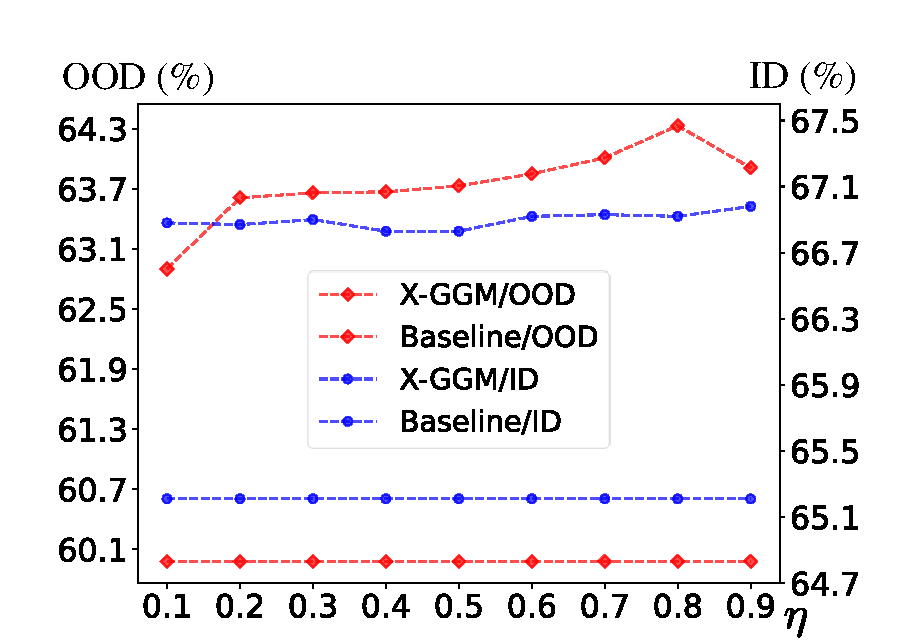
\includegraphics[width=1.\linewidth]{figure/c3_hp_1.pdf}
\subcaption{VQA-CP v2 ``Other''}
\label{fig:c3_abl_param_1}
\end{subfigure}
\begin{subfigure}[b]{0.495\linewidth}
\centering
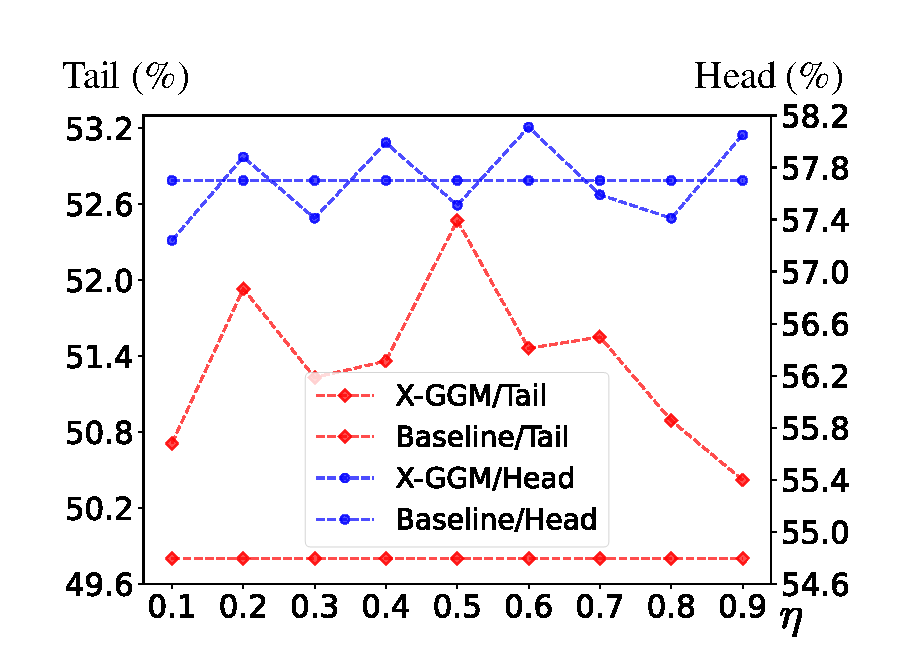
\includegraphics[width=1.\linewidth]{figure/c3_hp_2.pdf}
\subcaption{GQA-OOD}
\label{fig:c3_abl_param_2}
\end{subfigure}
\caption{在VQA-CP v2 ``Other''和GQA-OOD数据集上不同$\eta$值下OOD和ID性能比较}
\label{fig:c3_abl_params}
\end{figure}
% ********************************************************************

\subsubsection{超参的影响}
算法~\ref{alg:c3_ggm}中的阈值$\eta$决定了在每次训练迭代时,R-GGM和N-GGM被执行的概率。
为了分析$\eta$对X-GGM提升模型分布外泛化性能的影响,本章进行了关于不同$\eta$值的消融实验。
本章考虑以下$\eta$值,即,$\eta \in \{0.1, 0.2, \dots, 0.9\}$。
实验结果如图~\ref{fig:c3_abl_param_1} 和图~\ref{fig:c3_abl_param_2} 所示。
本章观察到在$\eta = 0.8$和$\eta$ = 0.5时,使用X-GGM训练基线视觉问答模型LXMERT分别在VQA-CP v2 ``Other''和GQA-OOD数据集上取得了最佳的分布外泛化性能。
在VQA-CP v2 ``Other''和GQA-OOD上的平均分布外泛化性能提升分别为$+3.76_{\pm 0.36}$和$+1.54_{\pm 0.59}$。比较分布外泛化的性能提升与分布外泛化性能的标准偏差,本章可以认为分布外性能波动很小,这证明了提出的X-GGM方案对超参数$\eta$是鲁棒的。


% ********************************************************************
\begin{figure}[!t]
\vspace{-3mm}
\begin{subfigure}[b]{1.0\textwidth}
\centering
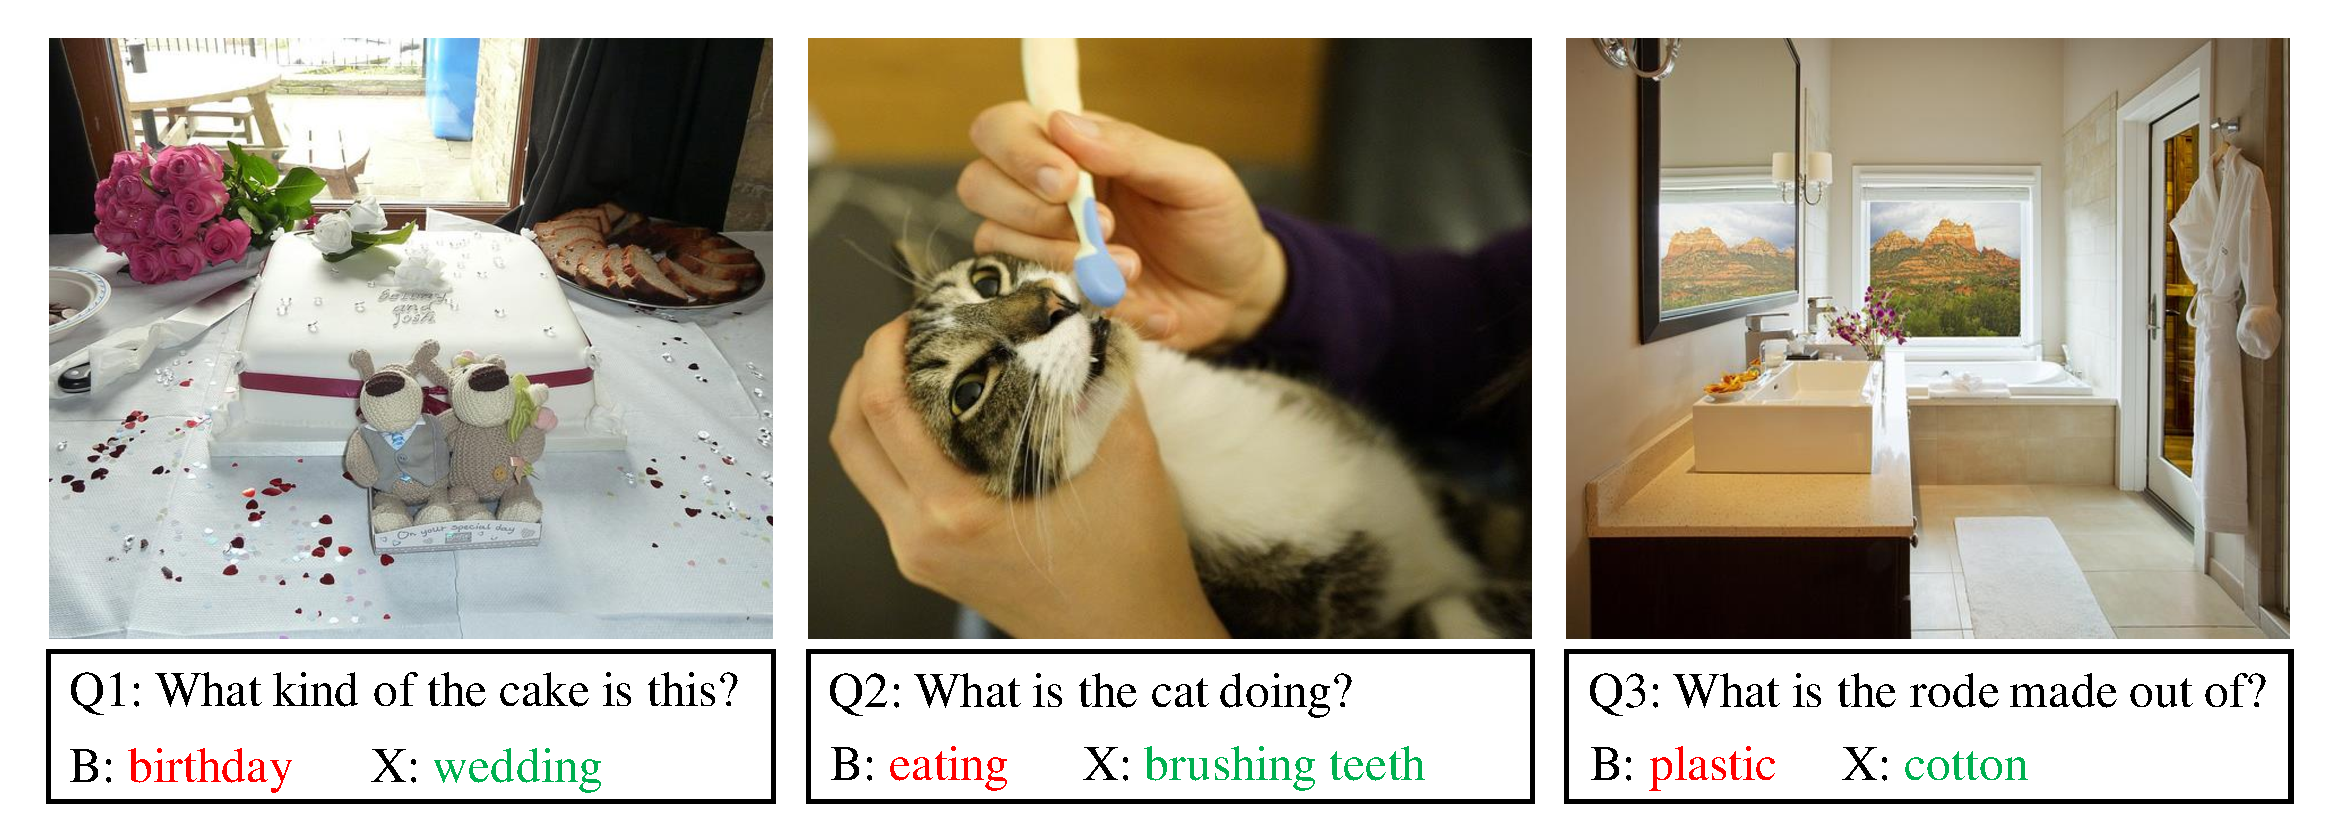
\includegraphics[width=0.95\linewidth]{figure/c3_vis_cp.pdf}
\subcaption{VQA-CP v2 OOD 测试集上答案预测举例}
\label{fig:c3_vis_cp}
\end{subfigure}
\begin{subfigure}[b]{1.0\textwidth}
\centering
\vspace{-1mm}
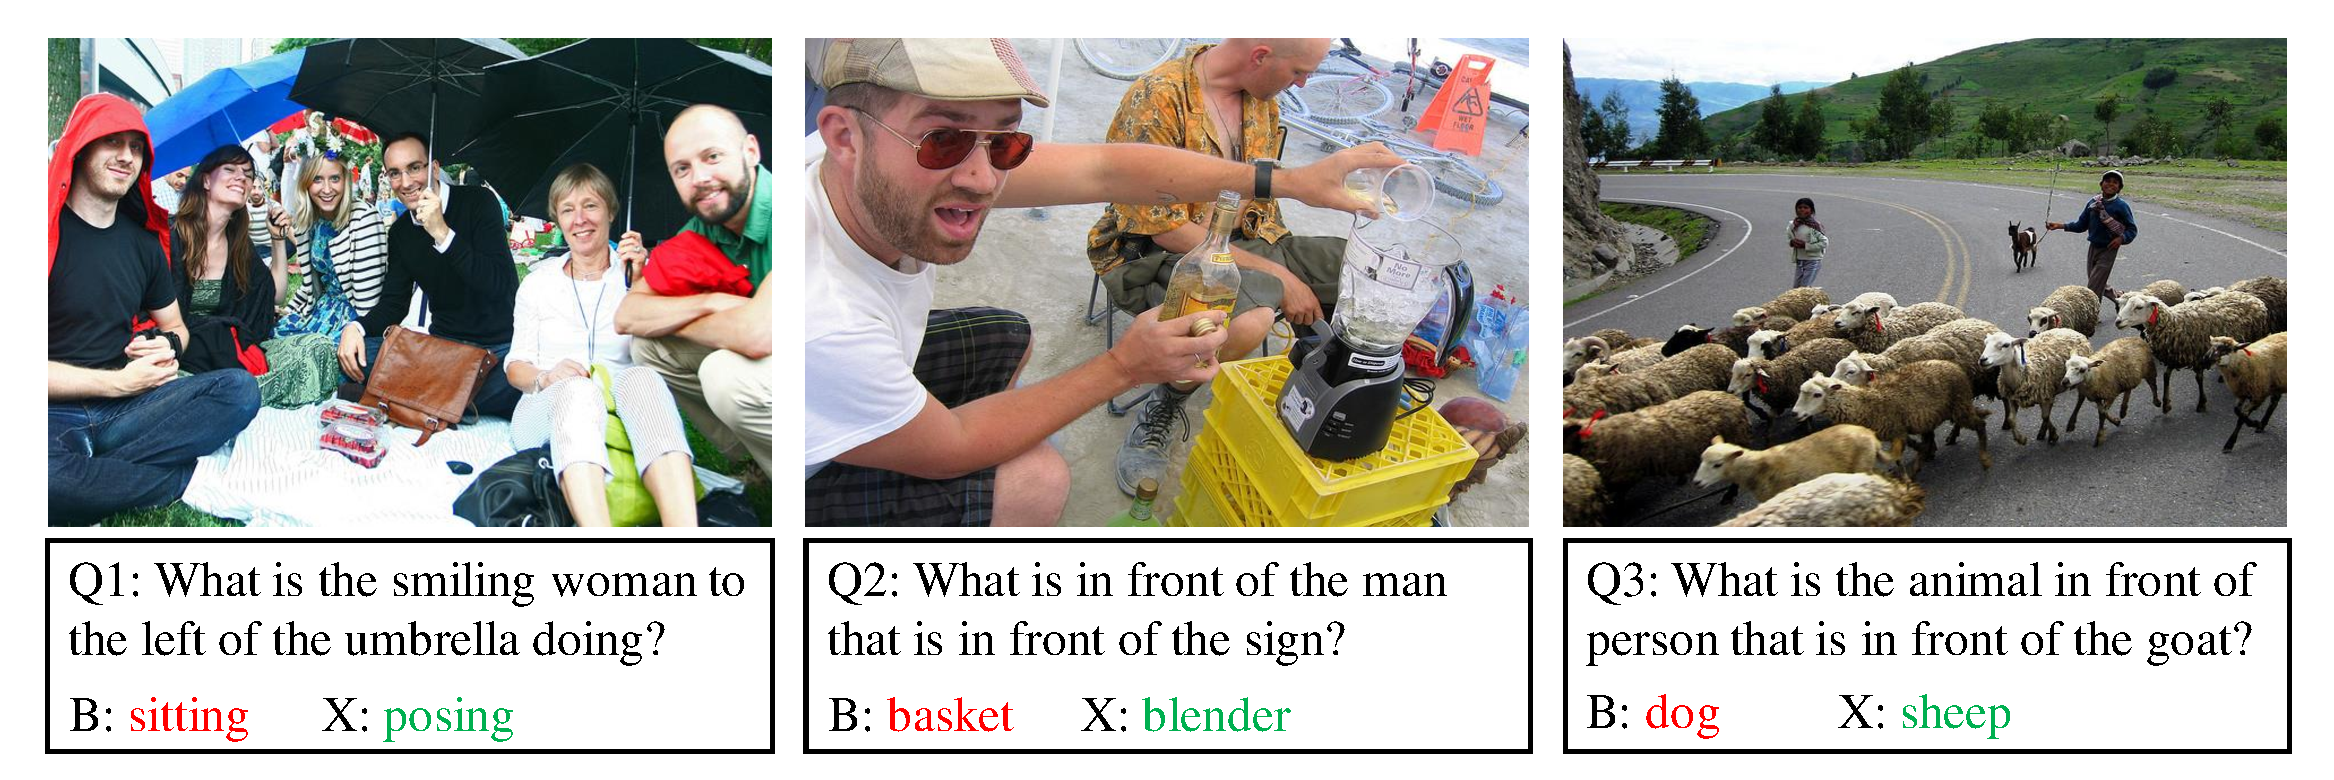
\includegraphics[width=0.95\linewidth]{figure/c3_vis_gqa.pdf}
\subcaption{GQA-OOD Tail 测试集上答案预测举例}
\label{fig:c3_vis_gqa}
\end{subfigure}
\vspace{-6mm}
\caption{在VQA-CP v2和GQA-OOD数据集的OOD测试集上的可视化举例
% 。B:基线视觉问答模型LXMERT;X:使用X-GGM训练的LXMERT。
% \textcolor{red}{错的}和\textcolor{ForestGreen}{对的}答案分别用\textcolor{red}{红色}和\textcolor{ForestGreen}{绿色}标出。
}
\label{fig:c3_vis_prediction}
\end{figure}
% ********************************************************************

% ********************************************************************
\begin{figure}[!t]
\centering
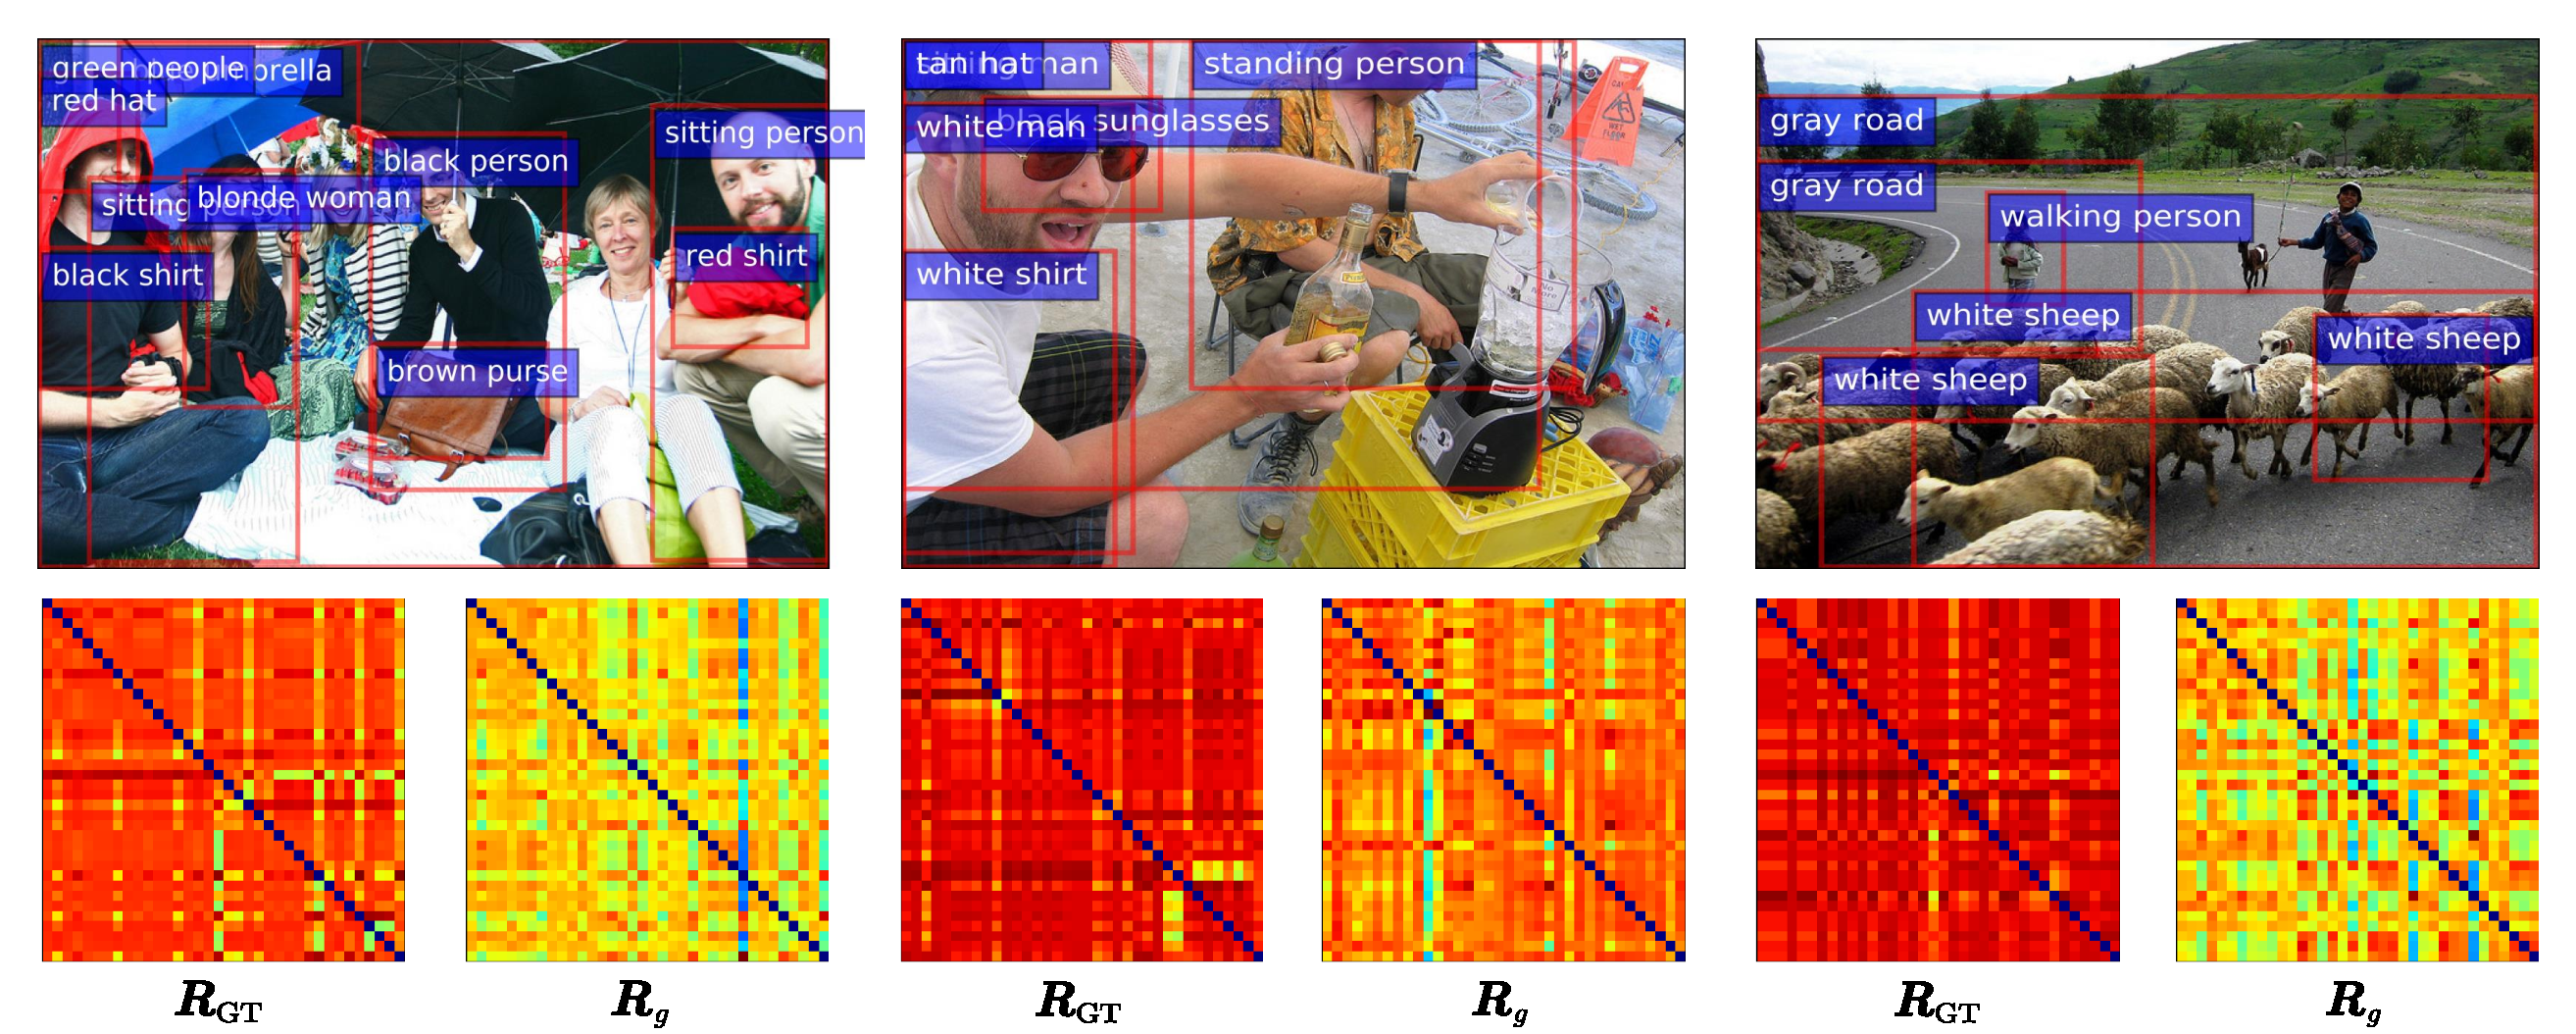
\includegraphics[width=0.95\linewidth]{figure/c3_vis_r.pdf}
\caption{在GQA-OOD Tail 测试集上关系矩阵热图可视化举例
% 。$\Rmat_{GT}$是预定义的关系矩阵真值,$\Rmat_{g}$是在R-GGM中生成的关系矩阵。
}
\label{fig:c3_vis_Rmat_additional}
\end{figure}
% ********************************************************************



% **************************************************************************
\xsubsection{定性实验}{Qualitative Experiment}

为了定性地说明X-GGM方案在提高基线视觉问答模型分布外泛化性能方面的有效性,图~\ref{fig:c3_vis_cp} 和图~\ref{fig:c3_vis_gqa} 分别展示了在VQA-CP v2和GQA-OOD的分布外测试集上的一些预测实例。
本章发现基线视觉问答模型LXMERT仍然倾向于使用域内的答案(如,\textit{eating}和\textit{sitting})来回答分布外的问题。
与之相反,使用X-GGM训练后的LXMERT则能生成如\textit{brushing teeth}和\textit{posing}这类分布外的答案。这表明使用X-GGM训练后,基线视觉问答模型LXMERT具有了更好的分布外泛化能力。
为了说明图生成建模的过程,考虑R-GGM中的关系生成过程,图~\ref{fig:c3_vis_Rmat_additional}比较了预定义的关系矩阵真值$\Rmat_{GT}$和生成的关系矩阵$\Rmat_{g}$的热图。
本章观察到$\Rmat_{g}$的热图中节点间的关系变得更具辨别性,并且在R-GGM之后生成了新的关系。




% **************************************************************************
\xsection{本章小结}{Summary} 

本章提出了一种全新的基于图生成建模的训练策略。
该策略以一定的概率交替地执行R-GGM和N-GGM来生成新的关系矩阵和新的节点表征,以此促使基线视觉问答模型能够泛化到分布外样本。
此外,为了缓解图对抗学习过程中的不稳定梯度问题,本章提出了一种梯度分布一致性损失来约束具有对抗性扰动的数据分布和生成的数据分布的梯度一致性。
广泛的实验表明本章提出的训练策略在不影响域内性能的情况下,能显著提高视觉问答模型的分布外泛化性能。
在未来,我们的目标是探索一种新的基于图生成模型的算法,该算法可以显式地编码图像中目标间的关系并明确地进行分布外的数据增强,以此来提高视觉问答模型分布外的泛化能力。


